\documentclass[main]{subfiles}


\begin{document}
\newpage
\section{Why Spikes}

Preface- This chapter (as most can tell by the title) deals with the advantages and disadvantages of using spikes (action potentials) in order to convey information. Traditional hardware computing uses binary 'steps': 0 to 1, GND to VND (strictly speaking the rising edge and falling edges of a step) to transfer information and this chapter will demonstrate why biological spikes are superior.


\subsection{What is a Neuronal Spike?}

By now most readers should be aware of how an action potential is generated and propagates through a neuron,but here is a short recap.

  \begin{figure}[H]
	\centering
	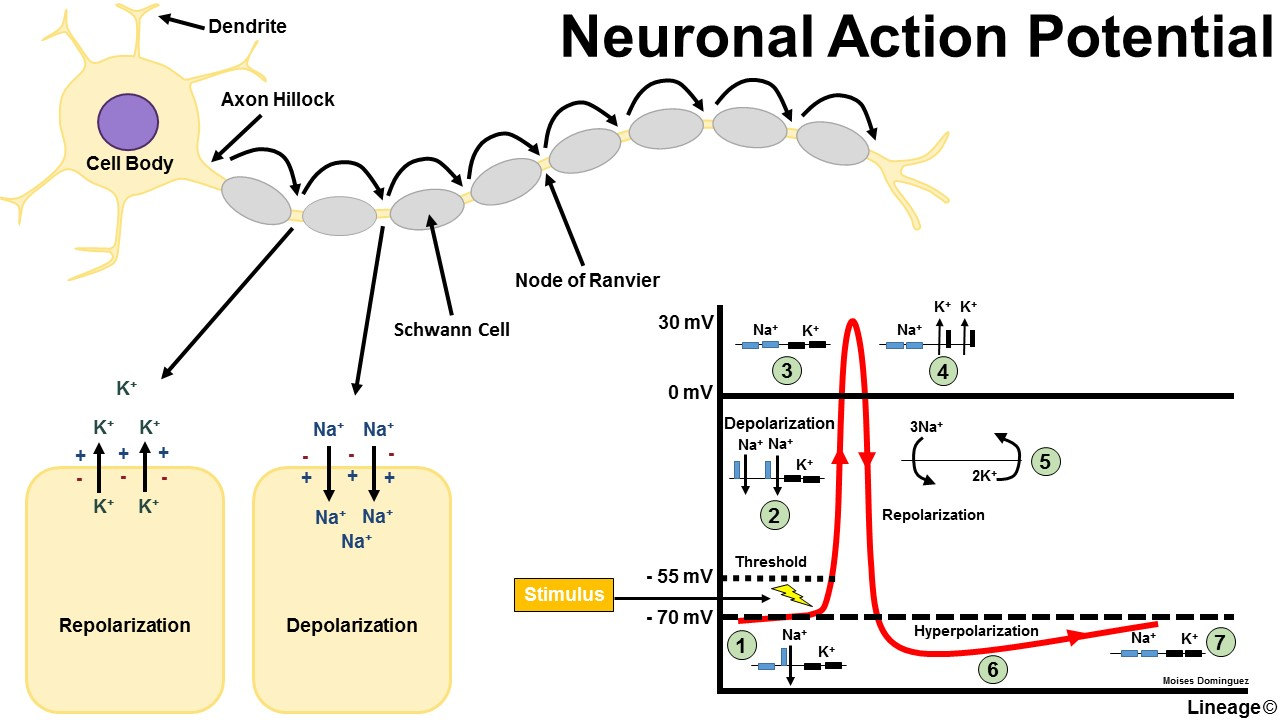
\includegraphics[width=0.9\linewidth]{09_WhySpikes/figures/neuronal action potential.jpg}
	\caption{Quick Action Potential Diagram.}
  \end{figure}

Step 1: Neuron is at resting potential (-70mV) which is determined by the balance between extracellular and intracellula K+, Na+. and Cl- concentrations (see later section for Hodgkin Huxley model)

Step 2: Neuron receives inputs at its dendrites which raises the membrane potential. If the membrane potential is below the threshold potential (~55mV), no AP is generated. If the resulting membrane potential is above the threshold, cell depolarization occurs.

Step 3: Voltage gated Na+ channels open causing Na+ influx into the cell which raises the membrane voltage which forces neighboring Na+ channels to also open. This continues up until a peak membrane potential of ~50mV.

Step 4: The Na+ channels begin to deactivate and voltage gated K+ channels begin to open causing K+ ion efflux. This rapidly lowers the membrane potential to below the baseline/resting potential levels (-80 ~ -90 mV) which is called hyper-polarization.

During this stage, the refractory period, the neuron is unable to fire again while the original ion balance/concentration is reestablished via Na+/K+ ATPases.

\subsection{Why does a neuron spike?}
\subsubsection{(Dis)advantages of digital (spike) vs. non-digital communication}

There are several disadvantages to sending digital signals along a channel.
One of them is quantization loss:

\begin{figure}[H]
	\centering
	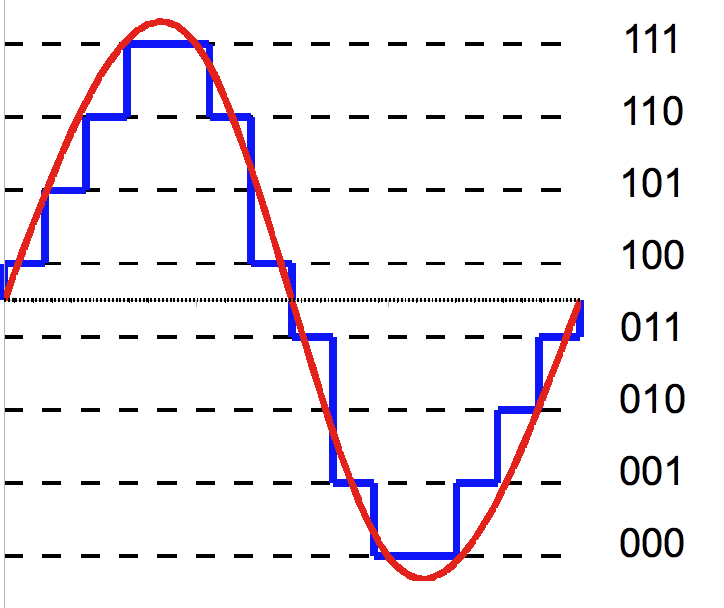
\includegraphics[width=0.9\linewidth]{09_WhySpikes/figures/3-bit_resolution_analog_comparison.png}
	\caption{Quantization error}
\end{figure}

As clearly seen- the output waveform (blue) is not perfectly in line with the original analogue input waveform (red). The calculation to determine quanta is straightforward.

As an aside- nonlinear quantization techniques and schemas exist. One can take advantage of alternative quantization techniques (below) to digitize an analogue signal that has a different entropy, or more information concentrated at lower values at the cost of reducing the resolution in higher values.

The most striking argument for Analogue activity is giving by Shannon's Information Capacity.
A calculation done for Crab neurons demonstrates that an analogue channel transfers 2,500~6,000 bits/s while a digital channel would have 50~220 bits/s: an order of magnitude inferior to an analogue channel


\subsubsection{Analogue communication in the Retina, C. Elegans, Locust}

Not every single neuron of every single creature is digital and spiking. There are several examples of species (C. Elegans, Cockroaches, Locusts) and even neuron families in mammals (Photo receptors, Horizontal cells, Olfactory Granule Cells) where neurons don't utilize spiking. 

An entire textbook (Neurones without Impulses- their significance for vertebrate and invertebrate nervous systems- Alan Roberts) exists to cover these example, but the lecture focuses on 1 case: C. Elegans.

C. Elegans has 302 neurons. None of them spike in the traditional AP generating manner. 

However recently, a group found spiking-"like" activity in an AWA (olfactory sensory) neuron type.


\begin{figure}[H]
	\centering
	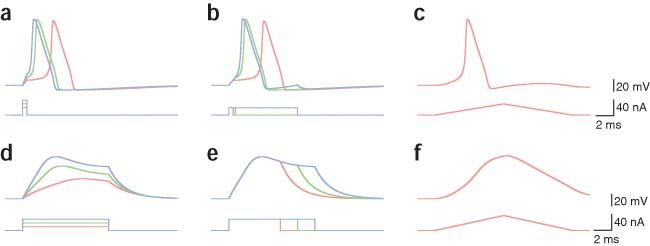
\includegraphics[width=0.9\linewidth]{09_WhySpikes/figures/celegans.jpg}
	\caption{Spiking LIKE activity in C elegans}
\end{figure}

\begin{figure}[H]
	\centering
	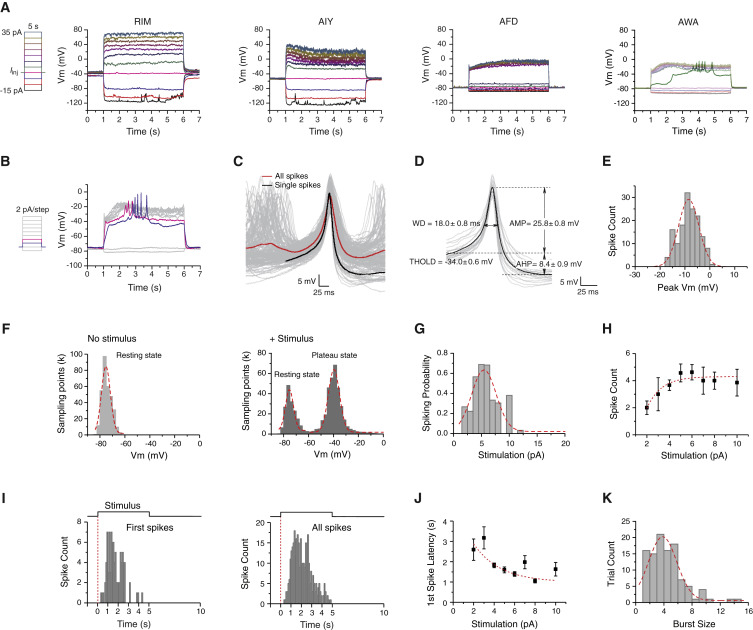
\includegraphics[width=0.9\linewidth]{09_WhySpikes/figures/celegans-different-neurons.jpg}
	\caption{Firing types in C elegans}
\end{figure}

After a series of back-and-forth arguments, this evidence proved to be inconclusive and the scientific consensus remains set on the fact that C Elegans neurons do not generate action potentials, but the resulting "graded" potentials are quite interesting.

\subsubsection{The different types of Action Potentials}

\subsection{Why Spike- from Biology?}
It has been demonstrated from a signal processing standpoint that digital spikes are inferior to analogue communications. It has also been demonstrated that there are insects that work perfectly well without spikes. So why use spikes?

Several reasons:

\begin{itemize}
	\item Spikes Synchronize Internal Processes
	-A paramecium (single celled organism) uses spikes to forcefully/instantly orient its motile cilia (motors) as part of avoidance behavior 
	\item Spikes send local information within a Cell
	-The ameoba uses Mechanosensetive Calcium channels to generate a spike which causes local contraction/compression to generate movement away from an object.
	\item Calcium spikes regulates homeostatic processes
	-Ca2+ intracellular signaling cascade/pathways are the foundations of molecular biology. Seeing Ca2+ influx follows an action potential, it would be wasteful to have to come up with a different mechanism to mediate Ca2+ levels. Spiking does this as a byproduct.
	\item Cells send information across long distances
	-Any analogue wavelength would decay over time, and be vulnurable to noise fluctuations. Neurons have tricks to reduce this (myelination, increasing axon diameter in sea squids), but ultimately spikes guarantee an intact and reconstructable signal being delivered. 
	\item Energy Efficiency
	-Self Explanatory. A human uses 100 Watts, the brain takes up 20W. Compare that to the power supply unit of a standard desktop (300W) or a high end rig (800W)
\end{itemize}


\subsection{How to measure spiking activity in a biological neuron?}

How would one measure a voltage level change of anything? Use a voltmeter!

The only caveat to this is probe design. Simply placing the tip of the probe in contact with the membrane is usually insufficient (especially at the 1~2 $\mu$meter level), thus there are several techniques to properly "clamp" the membrane.

\begin{figure}[H]
	\centering
	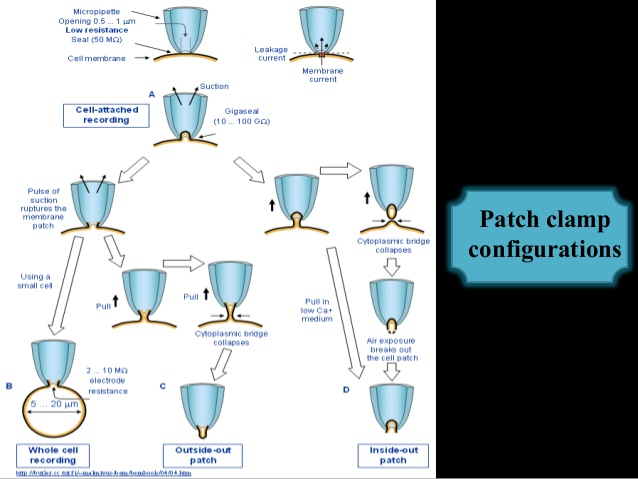
\includegraphics[width=0.9\linewidth]{09_WhySpikes/figures/patch-clam-technique-10-638.jpg}
	\caption{Patch Clamp configurations}
\end{figure}

Electrode design is actually quite a hardware challenge for electrical engineers and improvements are being made every year.


Alternatively Neuronal Spiking can be recorded via fluoresence techniques (Voltage Indicators)- Ace1Q-mNeon \& Ace2N-mNeon are examples. 

\begin{figure}[H]
	\centering
	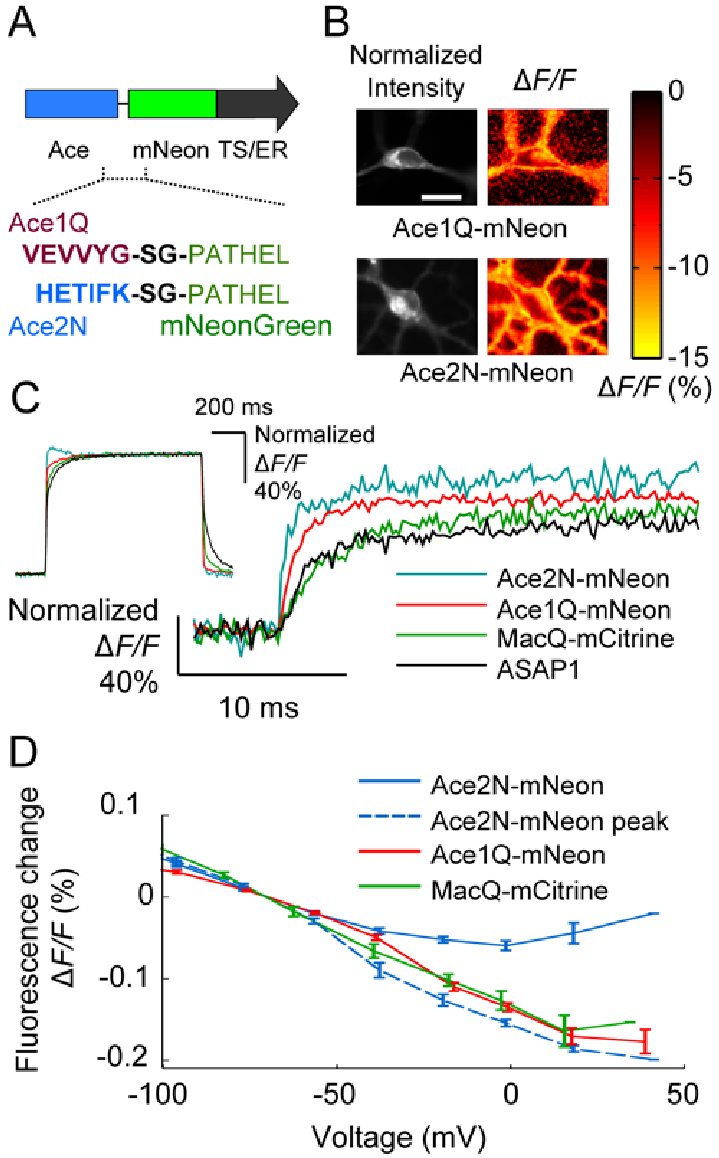
\includegraphics[width=0.9\linewidth]{09_WhySpikes/figures/Aceq.png}
	\caption{Voltage Indicators}
\end{figure}

GEVIs undergo a conformations change in response to a voltage change which changes their fluorescence levels. Several Examples are given
\begin{figure}[H]
	\centering
	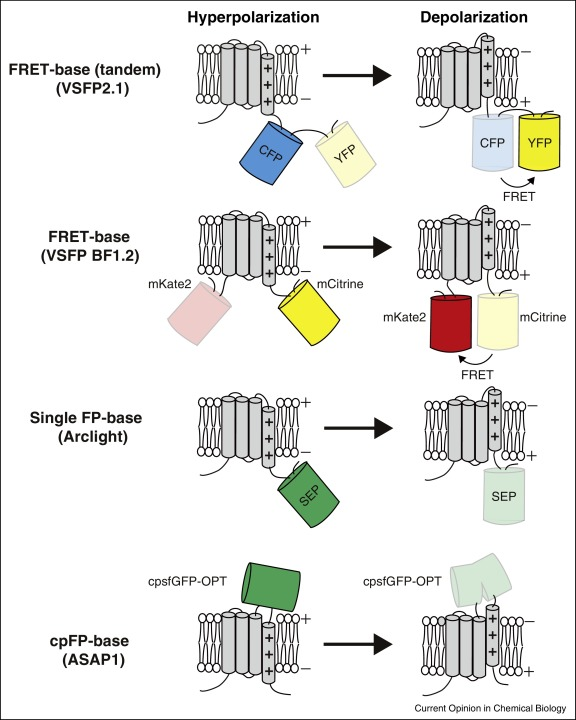
\includegraphics[width=0.9\linewidth]{09_WhySpikes/figures/GEVIs.jpg}
	\caption{More Voltage Indicators}
\end{figure}

Finally there are Calcium Indicators that do exactly the same thing but undergo a conformational shift in response to a change in intracellular calcium concentration.

\subsection{Temporal coding schemes with spikes}

Now that we've established that spikes are the method of information transportation in the brain, it is necessary to find a way to decode them.

There are several ways in which spiking data can encode information.

\begin{figure}[H]
	\centering
	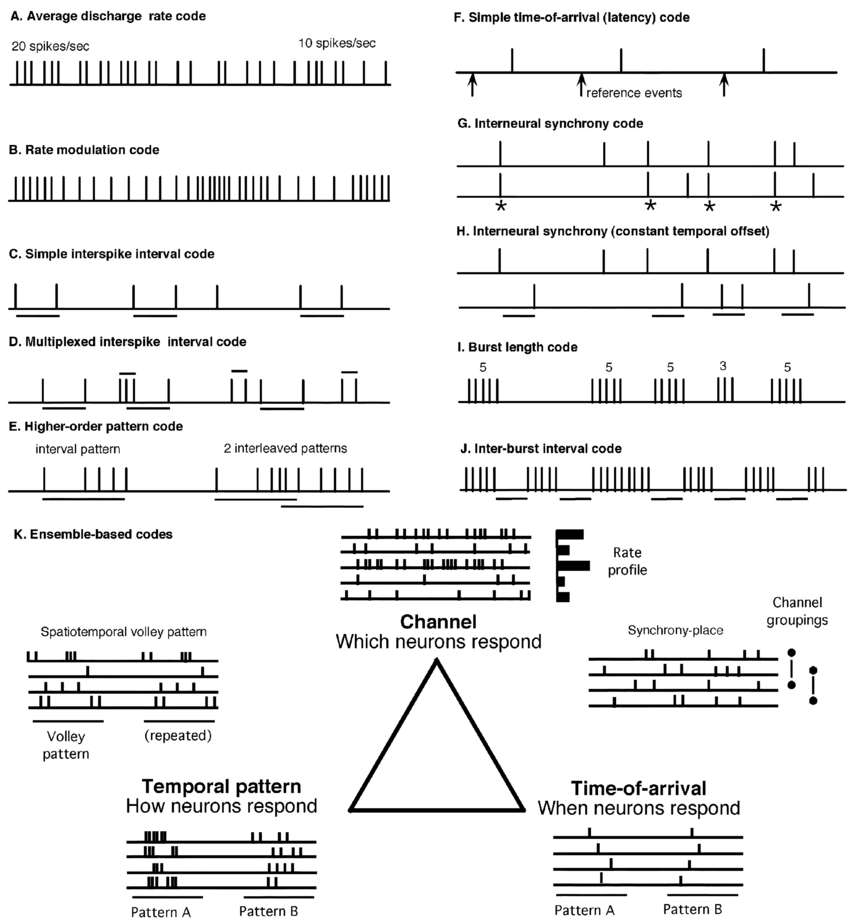
\includegraphics[width=0.9\linewidth]{09_WhySpikes/figures/TypesofSpikeCodings.png}
	\caption{Types of Spike Coding}
\end{figure}

These can be divided into 2 primary categories:
Rate coding (information = firing rate) and Temporal coding (information = time scheme)

The lecture gives several examples
\begin{itemize}
    \item Spike RATE coding in the Cat VI encodes direction selectivity
    \item Phase Coding in Place Cells in the Hippocampus to determine position
    \item Temporal (Latency) Coding to determine Interaural time difference 
\end{itemize}


\subsubsection{Deep Learning with "Time to first Spike"}

An Artifical Spiking Neural Network has been trained to utilize the time to first spike scheme.

The (MNIST) 2D image information was encoded in the following manner

\begin{figure}[H]
	\centering
	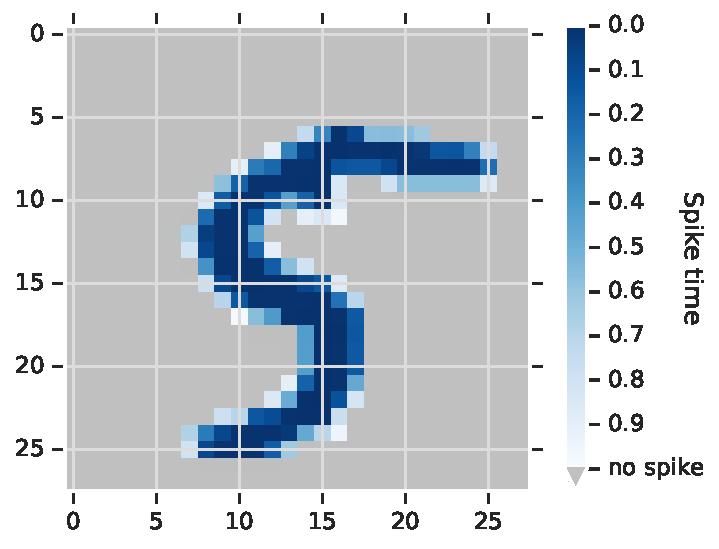
\includegraphics[width=0.9\linewidth]{09_WhySpikes/figures/figure2.pdf}
	\caption{TTFS Encoding of MNIST image}
\end{figure}

This paper modelled spikes via the Alpha Function

\begin{figure}[H]
	\centering
	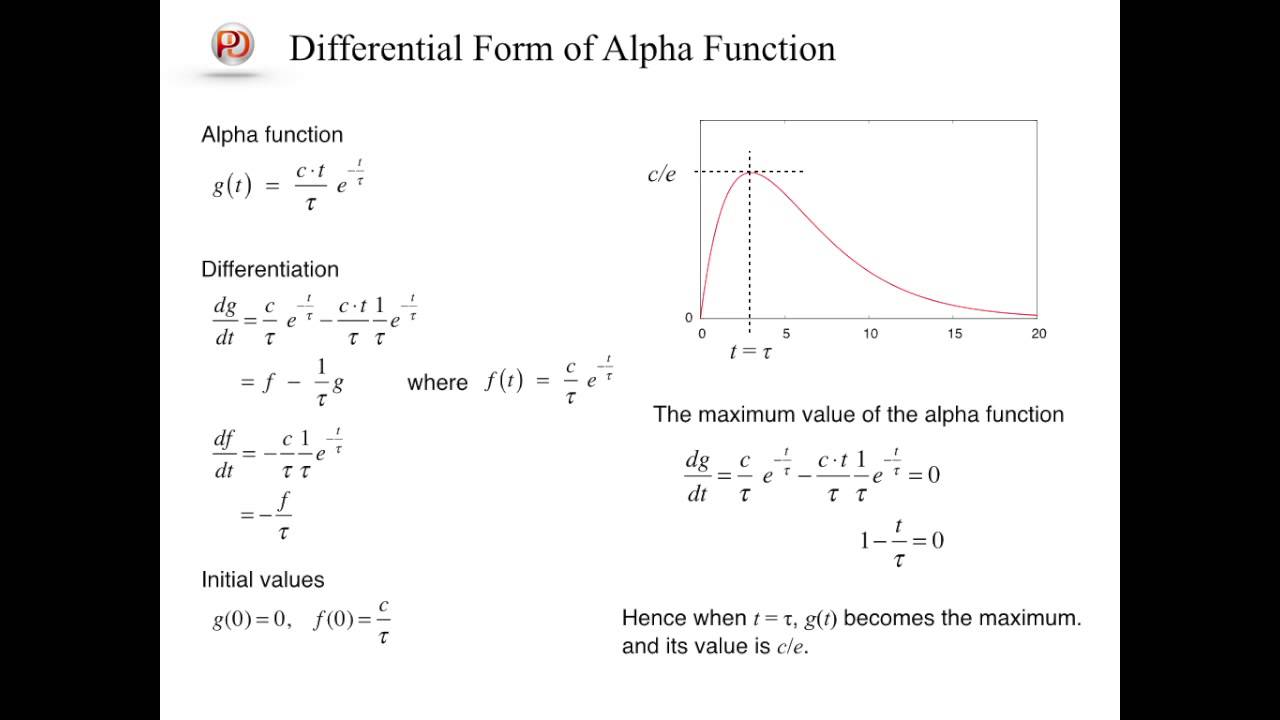
\includegraphics[width=0.9\linewidth]{09_WhySpikes/figures/whatsanalphafunction.jpg}
	\caption{Alpha Function}
\end{figure}

And it can be trained to solve Boolean tasks (AND, OR, XOR), as well as MNIST classification

\subsubsection{Hodgkin-Huxley Model}

Mathematically modelling neuronal firing can be done in different ways. The classic model is the Hodgkin-Huxley Model.

\begin{figure}[H]
	\centering
	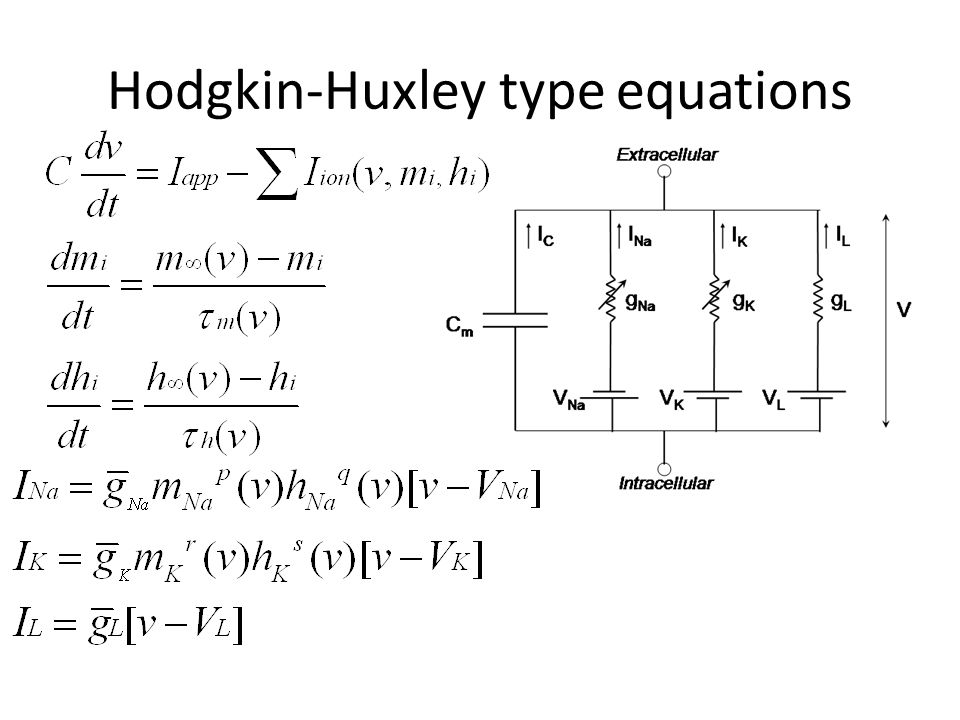
\includegraphics[width=0.9\linewidth]{09_WhySpikes/figures/Hodgkin-Huxley+type+equations.jpg}
	\caption{Hodgkin-Huxley}
\end{figure}

However multiple other models (Fitzhugh-Nagumo, Leaky Integrate \& Fire, Galves–Löcherbach, HTM models) exist and can be derived.

Keep in mind that these attempt to biologically model neurons, and not artificial neuron networks (ADALINE, MLP, McCulloch-Pitts Neurons, etc.)

\end{document}